\experiment{Binary Search}{08/11/2023}

\section{Aim}
Write a C program to read string data stored in a file. Sort the strings in alphabetical order
using Bubble Sort. Implement Binary Search to search for a given string. Implement sort and
search routines as separate functions.

\section{Algorithm}
 {\fontfamily{lmtt}\selectfont

  \subsection{Bubble Sort Function}
  Create a function \texttt{bubblesort(names, n)}:
  \begin{enumerate}[label=\arabic*:,left=0pt]
    \item \textbf{Start}
    \item Loop from \texttt{i} equal to 0 to \texttt{n - 1}:
          \begin{enumerate}[label=2.\arabic*:, start=1]
            \item Loop from \texttt{j} equal to 0 to \texttt{n - i - 1}:
                  \begin{enumerate}[label=2.1.\arabic*:, start=1]
                    \item If \texttt{strcmp(names[j], names[j + 1]) > 0}, then swap \texttt{names[j]} and \texttt{names[j + 1]}.
                  \end{enumerate}
          \end{enumerate}
    \item \textbf{Stop}
  \end{enumerate}

  \subsection{Binary Search Function}
  Create a function \texttt{binarysearch(names, n, x)}:
  \begin{enumerate}[label=\arabic*:,left=0pt]
    \item \textbf{Start}
    \item Set \texttt{l} to -1 and \texttt{r} to \texttt{n}.
    \item While \texttt{r - l > 1}:
          \begin{enumerate}[label=2.\arabic*:, start=1]
            \item Set \texttt{m} to \texttt{l + (r - l)/2}.
            \item If \texttt{strcmp(names[m], x) <= 0}, set \texttt{l} to \texttt{m}.
            \item Else, set \texttt{r} to \texttt{m}.
          \end{enumerate}
    \item Return \texttt{(l >= 0 \&\& strcmp(names[l], x) == 0) ? l : -1}.

    \item \textbf{Stop}
  \end{enumerate}

  \subsection{Main Function}
  In the \texttt{main} function:
  \begin{enumerate}[label=\arabic*:, start=1]
    \item \textbf{Start}
    \item Declare a 2D array \texttt{names[100][100]} to store names.
    \item Open the file \texttt{"studentname.txt"} in read mode (\texttt{"r"}).
    \item If the file does not exist, print "error" and return 0.
    \item Declare an integer variable \texttt{num} and initialize it to 0.
    \item Loop while reading names from the file using \texttt{fscanf(fp, "\%s", names[num])}:
          \begin{enumerate}[label=5.\arabic*:, start=1]
            \item Increment \texttt{num}.
          \end{enumerate}
    \item Close the file.
    \item Call the \texttt{bubblesort} function with \texttt{names} and \texttt{num} as arguments.
    \item Print "Sorted names:".
    \item Loop from \texttt{i} equal to 0 to \texttt{num - 1}:
          \begin{enumerate}[label=9.\arabic*:, start=1]
            \item Print \texttt{names[i]}.
          \end{enumerate}
    \item Declare a character array \texttt{searchname[100]}.
    \item Print "Enter name to search: ".
    \item Take user input for \texttt{searchname}.
    \item Call the \texttt{binarysearch} function with \texttt{names}, \texttt{num}, and \texttt{searchname} as arguments.
    \item If the result is not equal to -1, print "Found at position \texttt{result}".
    \item Else, print "Not found".
    \item Return 0.
    \item \textbf{Stop}
  \end{enumerate}
 }

\section{C Program}
\begin{lstlisting}[label={list:c_program:file_binary_search}]
#include <stdio.h>
#include <stdlib.h>
#include <string.h>

void bubblesort(char names[100][100], int n){
    for(int i = 0; i < n - 1; i++){
        for(int j = 0; j < n - i - 1; j++){
            if(strcmp(names[j], names[j + 1]) > 0){
                char temp[100];
                strcpy(temp, names[j]);
                strcpy(names[j], names[j + 1]);
                strcpy(names[j + 1], temp);
            }
        }
    }
}

int binarysearch(char names[100][100], int n, char *x){
    int l = -1, r = n;
    while(r - l > 1){
        int m = l + (r - l)/2;
        if(strcmp(names[m], x) <= 0) l = m;
        else r = m;
    }
    return (l >= 0 && strcmp(names[l], x) == 0)? l: -1;
}

int main(){
    char names[100][100];
    FILE *fp = fopen("studentname.txt", "r");
    if(!fp){
        printf("error\n");
        return 0;
    }

    int num = 0;
    while(fscanf(fp, "%s", names[num]) == 1){
        num++;
    }
     
    fclose(fp);
    bubblesort(names, num);

    printf("Sorted names: \n");
    for(int i = 0; i < num; i++){
        printf("%s\n", names[i]);
    }

    char searchname[100];
    printf("enter name to search: ");
    scanf("%s", searchname);
    int result = binarysearch(names, num, searchname); 

    if(result != -1){
        printf("found at position %d\n", result);
    }
    else{
        printf("not found\n");
    }

    return 0;
}

\end{lstlisting}

\section{Output}
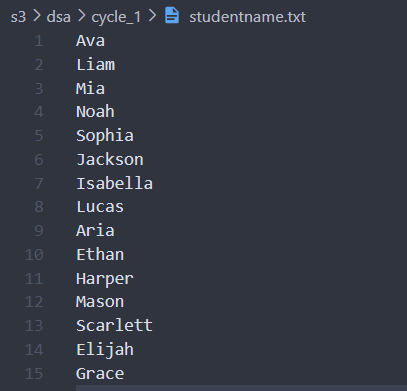
\includegraphics[]{Cycle_1/Outputs/BinarySearch2.png}
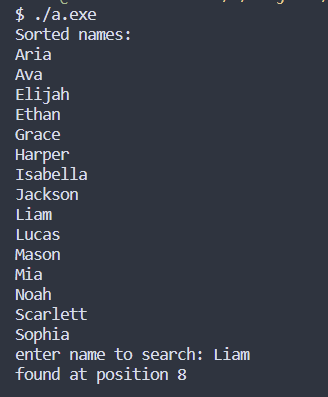
\includegraphics[]{Cycle_1/Outputs/BinarySearch1.png}

\section{Result}
Binary Search algorithm implemented. The program was executed and output verified.